\documentclass[12pt, titlepage]{article}

\usepackage{fullpage}
\usepackage[round]{natbib}
\usepackage{multirow}
\usepackage{booktabs}
\usepackage{tabularx}
\usepackage{graphicx}
\usepackage{float}
\usepackage{hyperref}
\usepackage{makecell}

\hypersetup{
	colorlinks,
	citecolor=blue,
	filecolor=black,
	linkcolor=red,
	urlcolor=blue
}

%% Comments

\usepackage{color}

\newif\ifcomments\commentstrue %displays comments
%\newif\ifcomments\commentsfalse %so that comments do not display

\ifcomments
\newcommand{\authornote}[3]{\textcolor{#1}{[#3 ---#2]}}
\newcommand{\todo}[1]{\textcolor{red}{[TODO: #1]}}
\else
\newcommand{\authornote}[3]{}
\newcommand{\todo}[1]{}
\fi

\newcommand{\wss}[1]{\authornote{blue}{SS}{#1}} 
\newcommand{\plt}[1]{\authornote{magenta}{TPLT}{#1}} %For explanation of the template
\newcommand{\an}[1]{\authornote{cyan}{Author}{#1}}

%% Common Parts

\newcommand{\progname}{Sayyara}
\newcommand{\authname}{Team 3, Tiny Coders
	\\ Arkin Modi
	\\ Joy Xiao
	\\ Leon So
	\\ Timothy Choy} % AUTHOR NAMES

\usepackage{hyperref}
\hypersetup{colorlinks=true, linkcolor=blue, citecolor=blue, filecolor=blue,
	urlcolor=blue, unicode=false}
\urlstyle{same}

\usepackage{parskip}
\usepackage{geometry}
\geometry{a4paper, portrait, margin=1in}



\begin{document}

\title{System Design for \progname{}}
\author{\authname}
\date{\today}

\maketitle

\pagenumbering{roman}

\section{Revision History}

\begin{table}[hp]
	\caption{Revision History} \label{TblRevisionHistory}
	\begin{tabularx}{\textwidth}{llX}
		\toprule
		\textbf{Date}     & \textbf{Developer(s)} & \textbf{Change}                                  \\
		\midrule
		December 28, 2022 & Arkin Modi            & Revision History \& Mark Not Applicable Sections \\
		January 7, 2023   & Joy Xiao              & Introduction \& Purpose                          \\
		January 11, 2023  & Leon So               & Undesired Event Handling                         \\
		January 12, 2023  & Leon So               & Normal Behaviour \& Introduction                 \\
		January 16, 2023  & Joy Xiao              & Component Diagram                                \\
		January 17, 2023  & Arkin Modi            & Create Timeline                                  \\
		January 17, 2023  & Arkin Modi            & Add Work Order Mockups                           \\
		January 17, 2023  & Joy Xiao              & Add Mockups                                      \\
		January 17, 2023  & Leon So               & Add Mockups                                      \\
		January 17, 2023  & Timothy Choy          & Add Mockups                                      \\
		\bottomrule
	\end{tabularx}
\end{table}

\newpage

\section{Reference Material}

This section records information for easy reference.

\subsection{Abbreviations and Acronyms}

\begin{tabular}{l l}
	\toprule
	\textbf{symbol} & \textbf{description}            \\
	\midrule
	\progname       & Explanation of program name     \\
	MIS             & Module Interface Specifications \\
	MG              & Module Guide                    \\
	\bottomrule
\end{tabular}

\newpage

\tableofcontents

\newpage

\listoftables

\listoffigures

\newpage

\pagenumbering{arabic}

\section{Introduction}

The following document details the System Design for project Sayyara. Sayyara is a progressive web
application (PWA) which will act as a single platform for independent auto repair shops and vehicle
owners. This platform will allow independent auto repair shops and vehicle owners to interact in a
more efficient and effective manner.

Complementary documents include the Module Interface Specifications and Module Guide. The full
documentation and implementation can be found at
\url{https://github.com/arkinmodi/project-sayyara/}.

\section{Purpose}

The purpose of this document is to display the component decomposition of the system and provide
the user interface designs of the software being built. The implementation of the software will be
based off of the designs within this document. The MIS
\url{https://github.com/arkinmodi/project-sayyara/blob/main/docs/Design/SoftDetailedDes/MIS.pdf}
and MG
\url{https://github.com/arkinmodi/project-sayyara/blob/main/docs/Design/SoftArchitecture/MG.pdf}
are also created to give details to the software architecture and detailed component breakdowns for
the project.

\section{Scope}

\wss{Include a figure that show the System Context (showing the boundary between
	your system and the environment around it.)}

\section{Project Overview}

\subsection{Normal Behaviour}
Sayyara is an event-driven application which handles inputs from the intended users including:
vehicle owners, and independent auto repair shop owners and employees. The application will accept
various inputs through a variety of input forms and controls. Under normal behaviour where valid
inputs are entered and valid events are triggered, the application will: update the appropriate
local and global application states, trigger the corresponding side-effects, and/or update the
database accordingly.

Vehicle owners can search for auto repair shops and services; request quotes for service; book,
view, and manage service appointments and work orders. On the application, auto repair shop owners
will be able to manage a list of employees; manage a list of service types and corresponding
service appointment availabilities; manage store information such as location, hours of operation,
and contact information. Auto repair shop owners and employees will be able to view and manage
quotes, service appointments, and work orders.

\subsection{Undesired Event Handling}

Undesired events will be handled both client-side and server-side.

On the client-side, if an unexpected event arises or the application enters a bad state, the
application will reset to a safe state. For example, if a user attempts to access a route that they
are not authorized to access, they will be either redirected to an appropriate route, prompted to
login, or an error page will be displayed with instructions to return to the home page. Input forms
will also include input validation to ensure only properly formed data is handled. If the user
attempts to input invalid data, the form field will reset and form submission will be blocked. The
user will be prompted to enter a valid input value in the form field. Similarly, various user
actions and inputs that may pose cause that the application to enter an undesirable state will be
validated before updating the application state.

On the server-side, each API will return a response with the appropriate error status code and
message. Subsequently, the client will have logic to gracefully handle unsuccessful responses and
status codes, preventing the system from entering an undesirable state. Inputs will also be
validated on the server-side by parsing the input data using defined schemas. This will ensure data
integrity and prevents the undesirable data from entering the workflows or database.

\subsection{Component Diagram}

\begin{figure}[H]
	\centering
	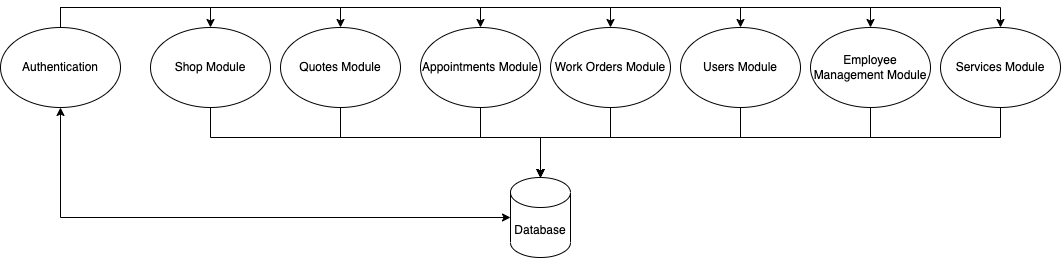
\includegraphics[width=\textwidth]{component-diagram.png}
	\caption{Component Diagram}
	\label{ComponentDiagram}
\end{figure}

\subsection{Connection Between Requirements and Design} \label{SecConnection}

\wss{The intention of this section is to document decisions that are made
	``between'' the requirements and the design.  To satisfy some requirements,
	design decisions need to be made.  Rather than make these decisions implicit,
	they are explicitly recorded here.  For instance, if a program has security
	requirements, a specific design decision may be made to satisfy those
	requirements with a password.}

\section{System Variables}
\subsection{Monitored Variables}
N/A

\subsection{Controlled Variables}
N/A

\subsection{Constants Variables}
N/A

\section{User Interfaces}

% \wss{Design of user interface for software and hardware.  Attach an appendix if
% 	needed. Drawings, Sketches, Figma}

\subsection{Home Page}

\begin{figure}[H]
	\centering
	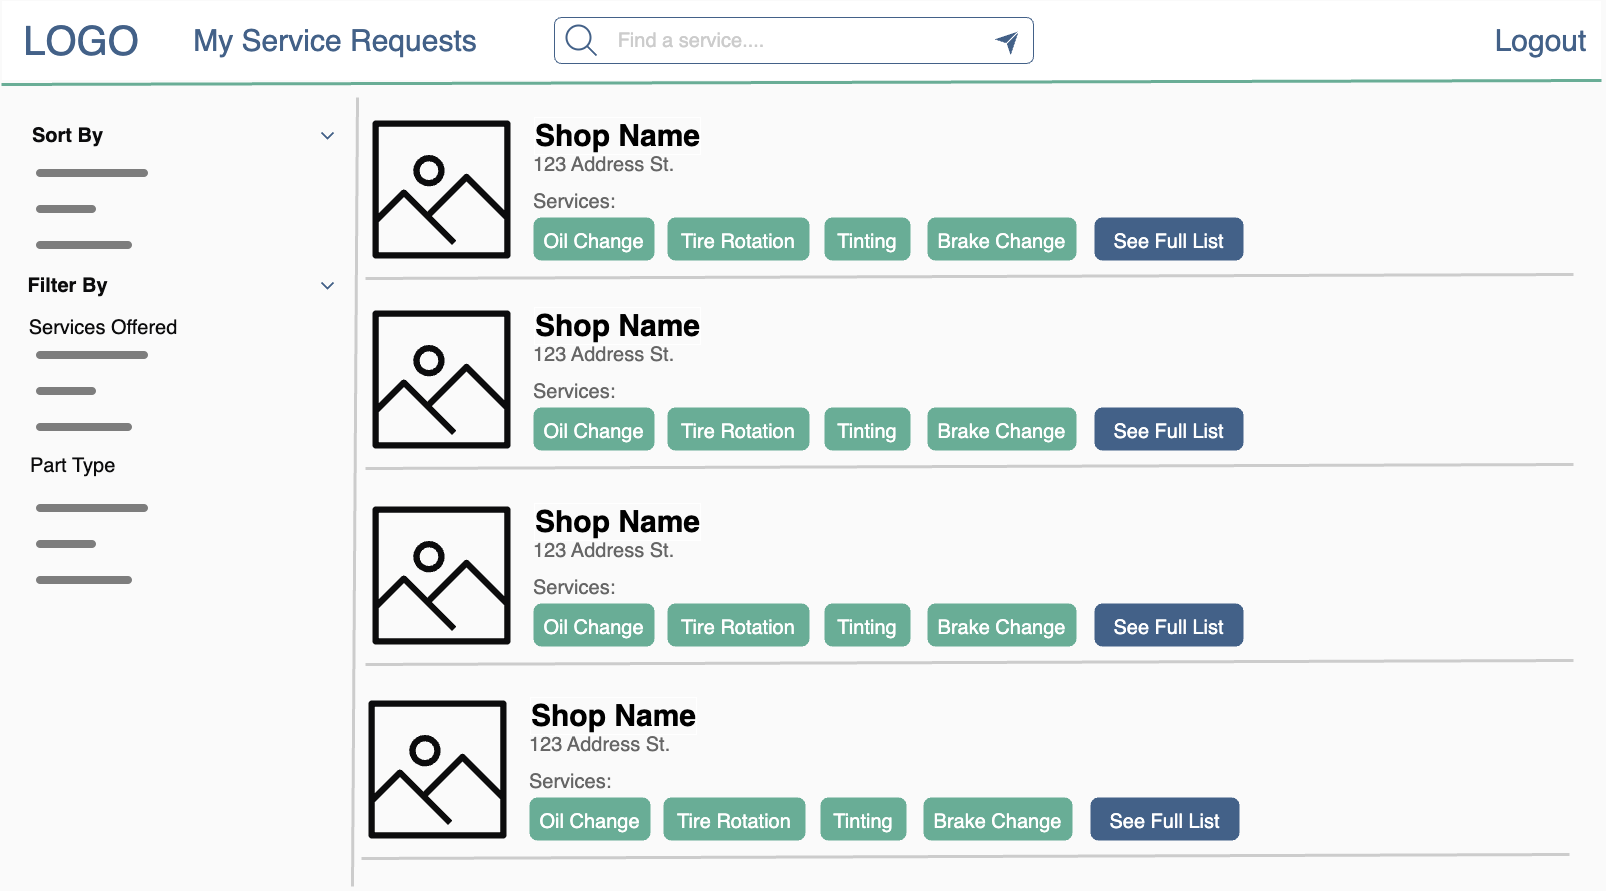
\includegraphics[width=\textwidth]{mockups/Home Page (Logged In) (Desktop).png}
	\caption{Home Page \textemdash{} Logged In (Desktop)}
\end{figure}

\begin{figure}[H]
	\centering
	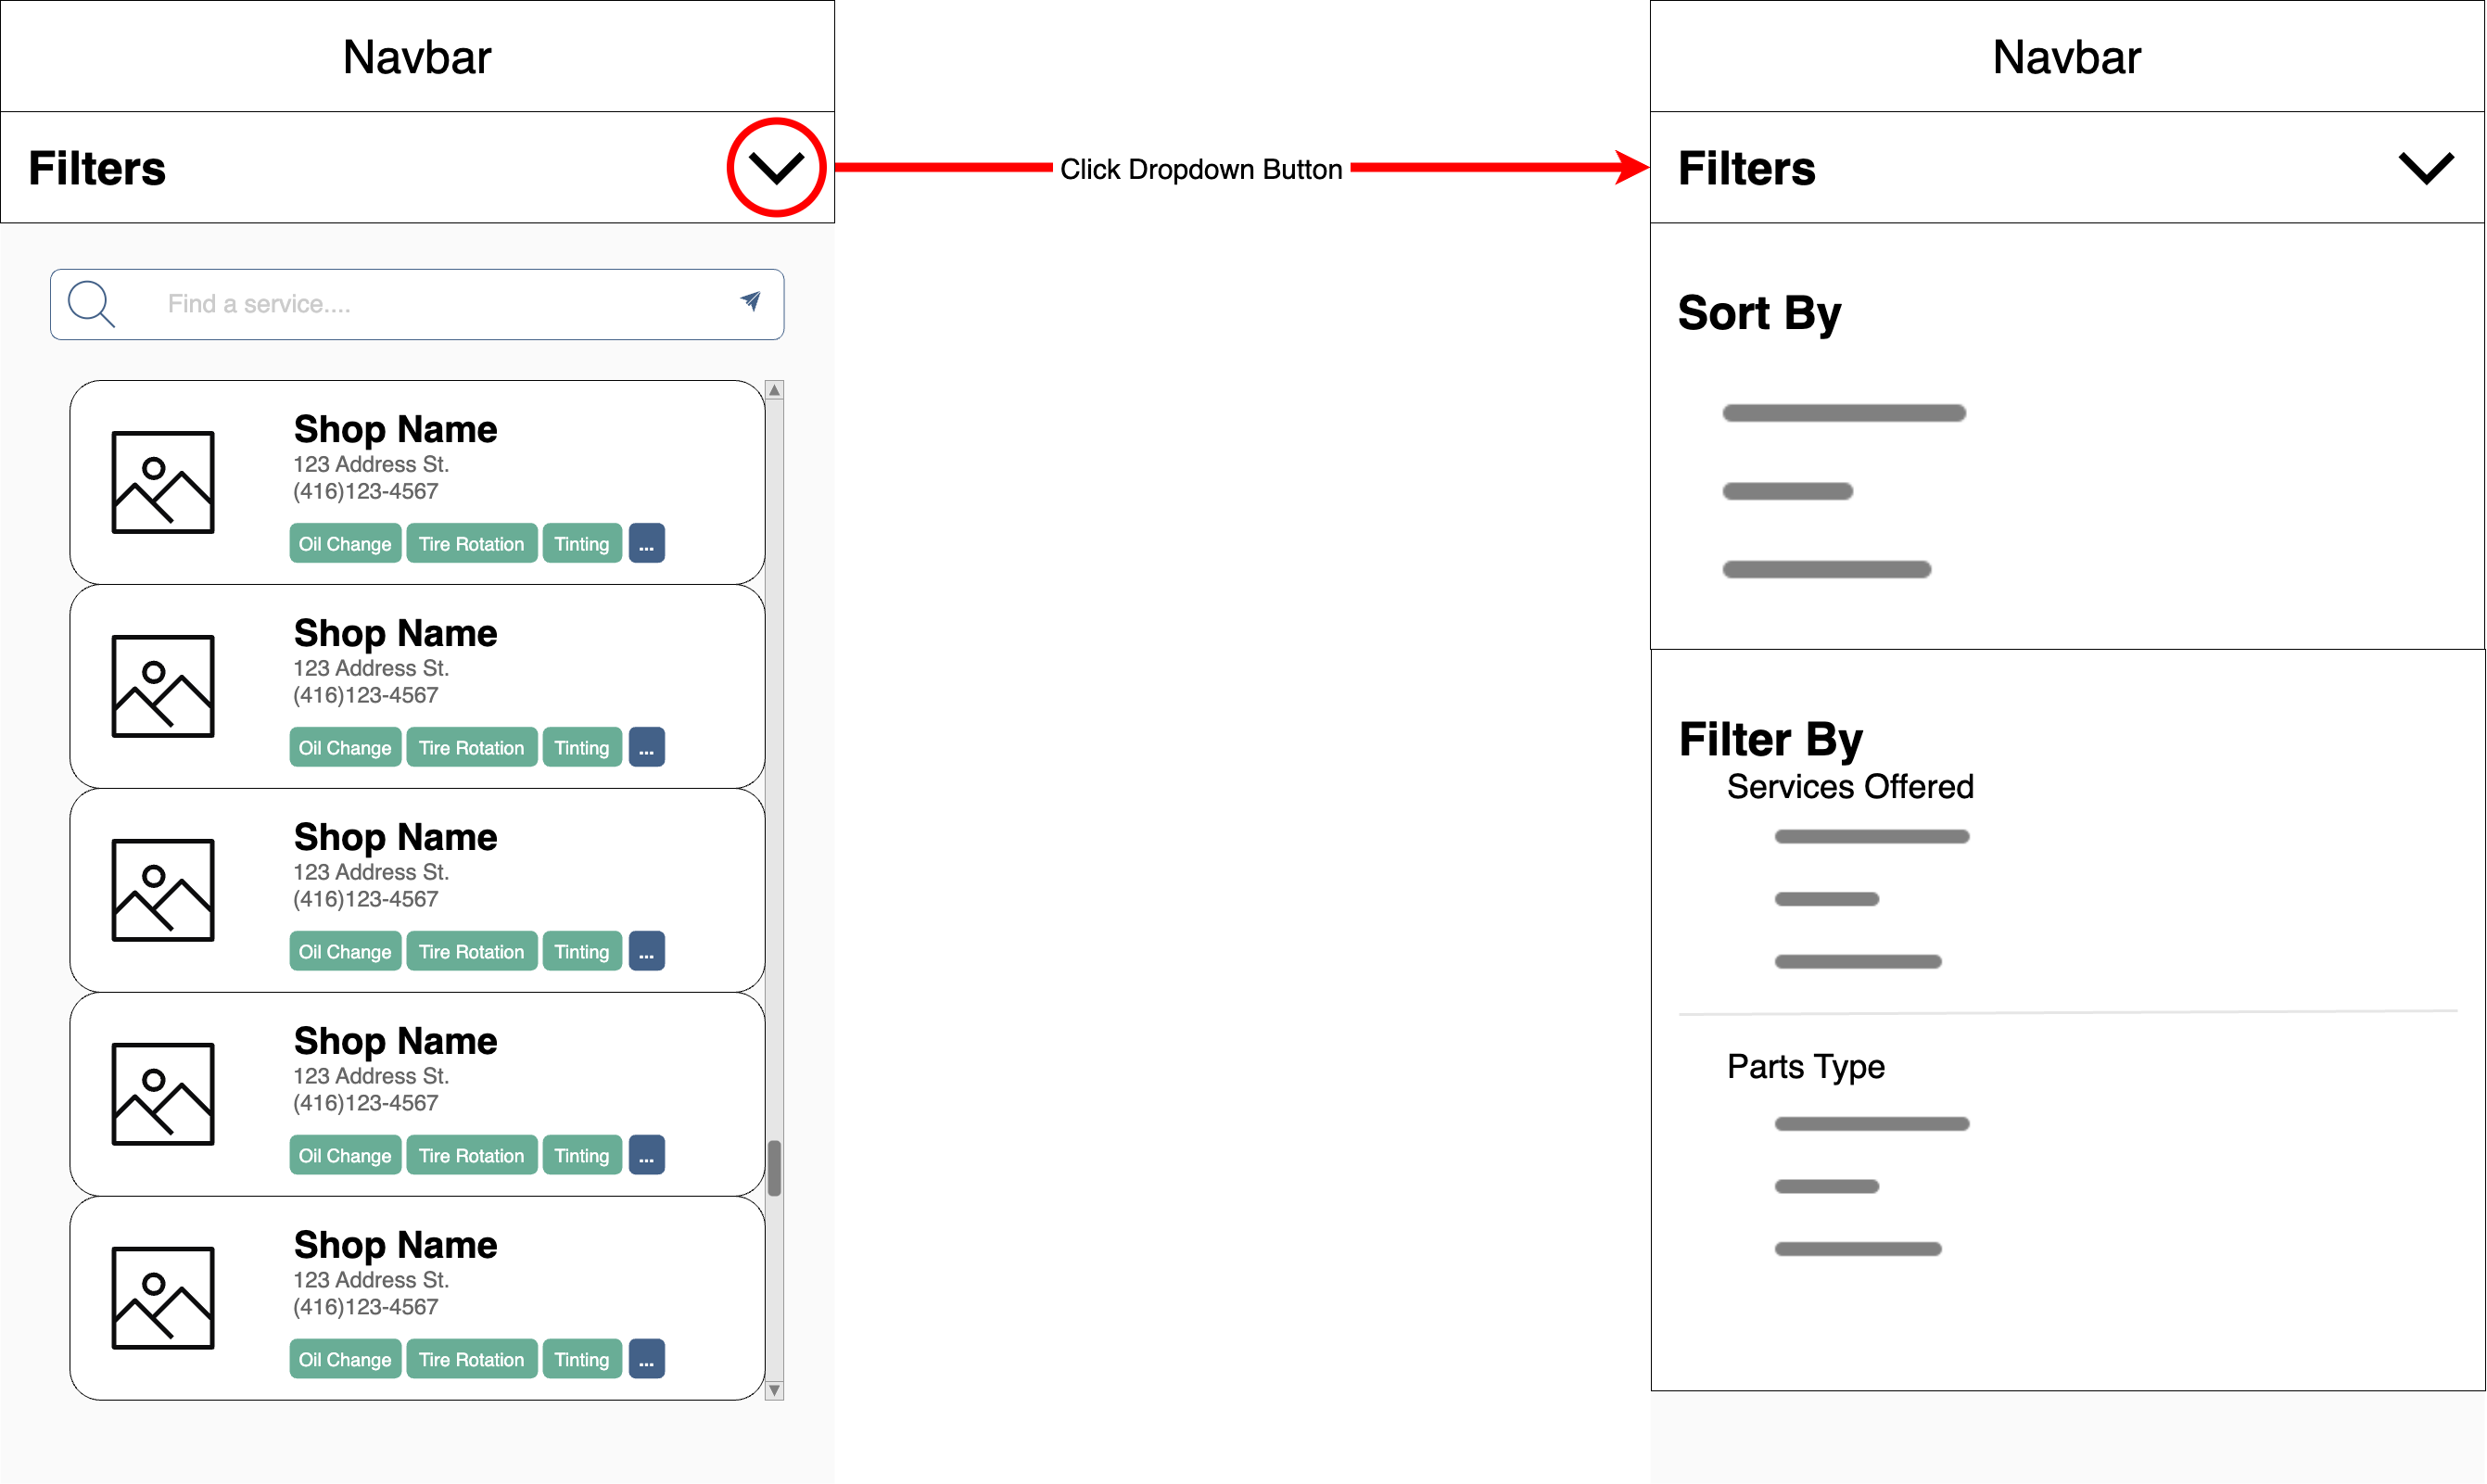
\includegraphics[width=\textwidth]{mockups/Home Page (Mobile).png}
	\caption{Home Page \textemdash{} Logged In (Mobile)}
\end{figure}

\subsection{Manage Shop Employees}

\begin{figure}[H]
	\centering
	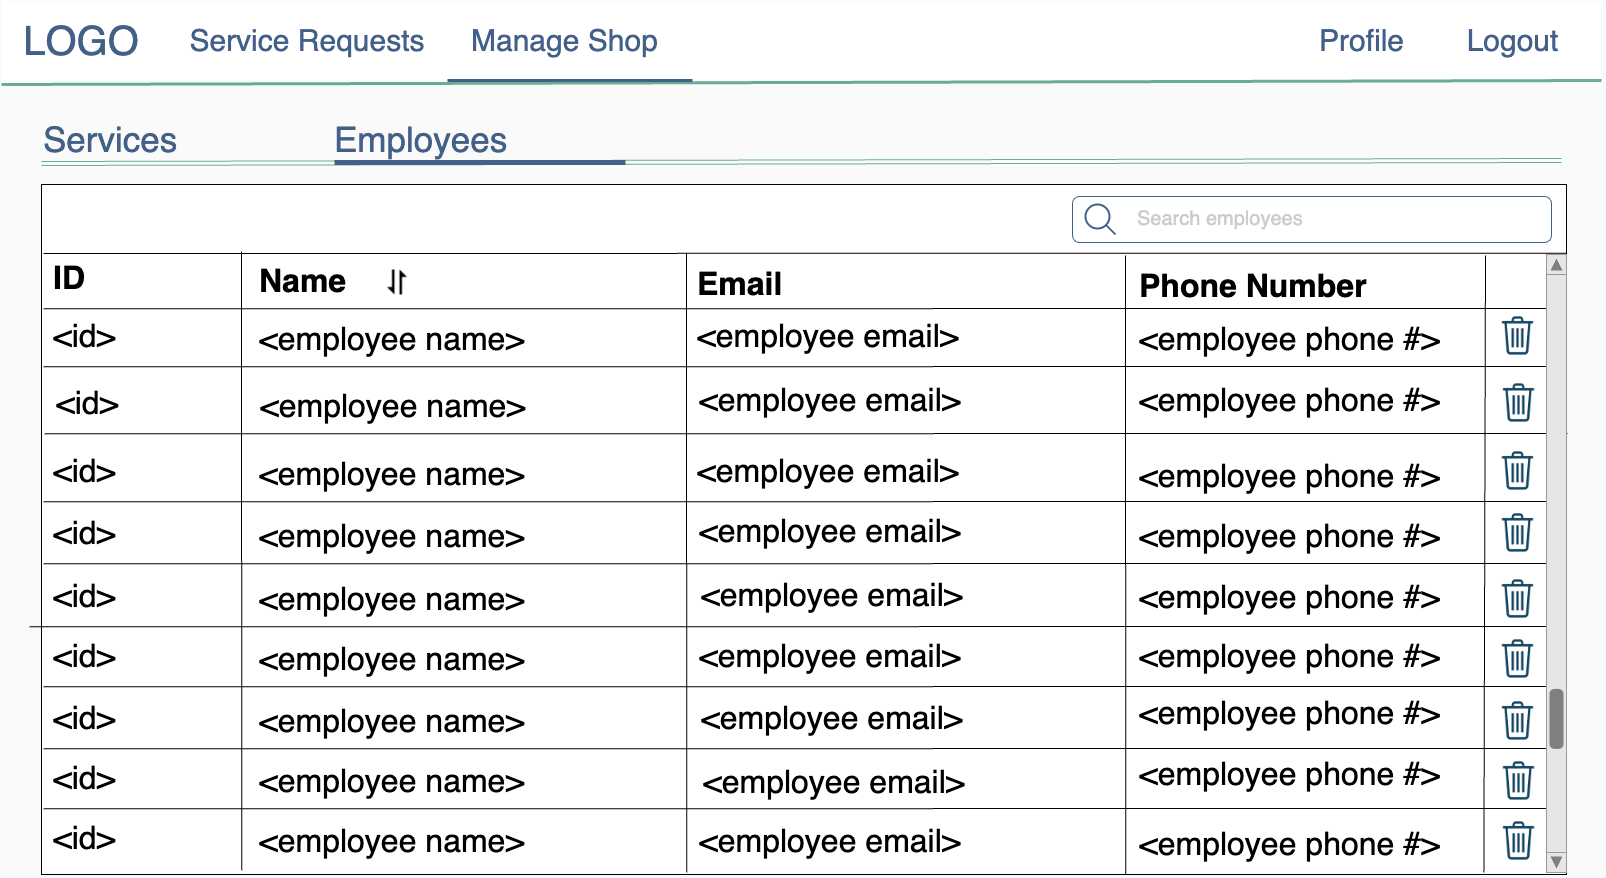
\includegraphics[width=\textwidth]{mockups/Manage Shop (Employees) (Desktop).png}
	\caption{Manage Shop \textemdash{} Employees (Desktop)}
\end{figure}

\begin{figure}[H]
	\centering
	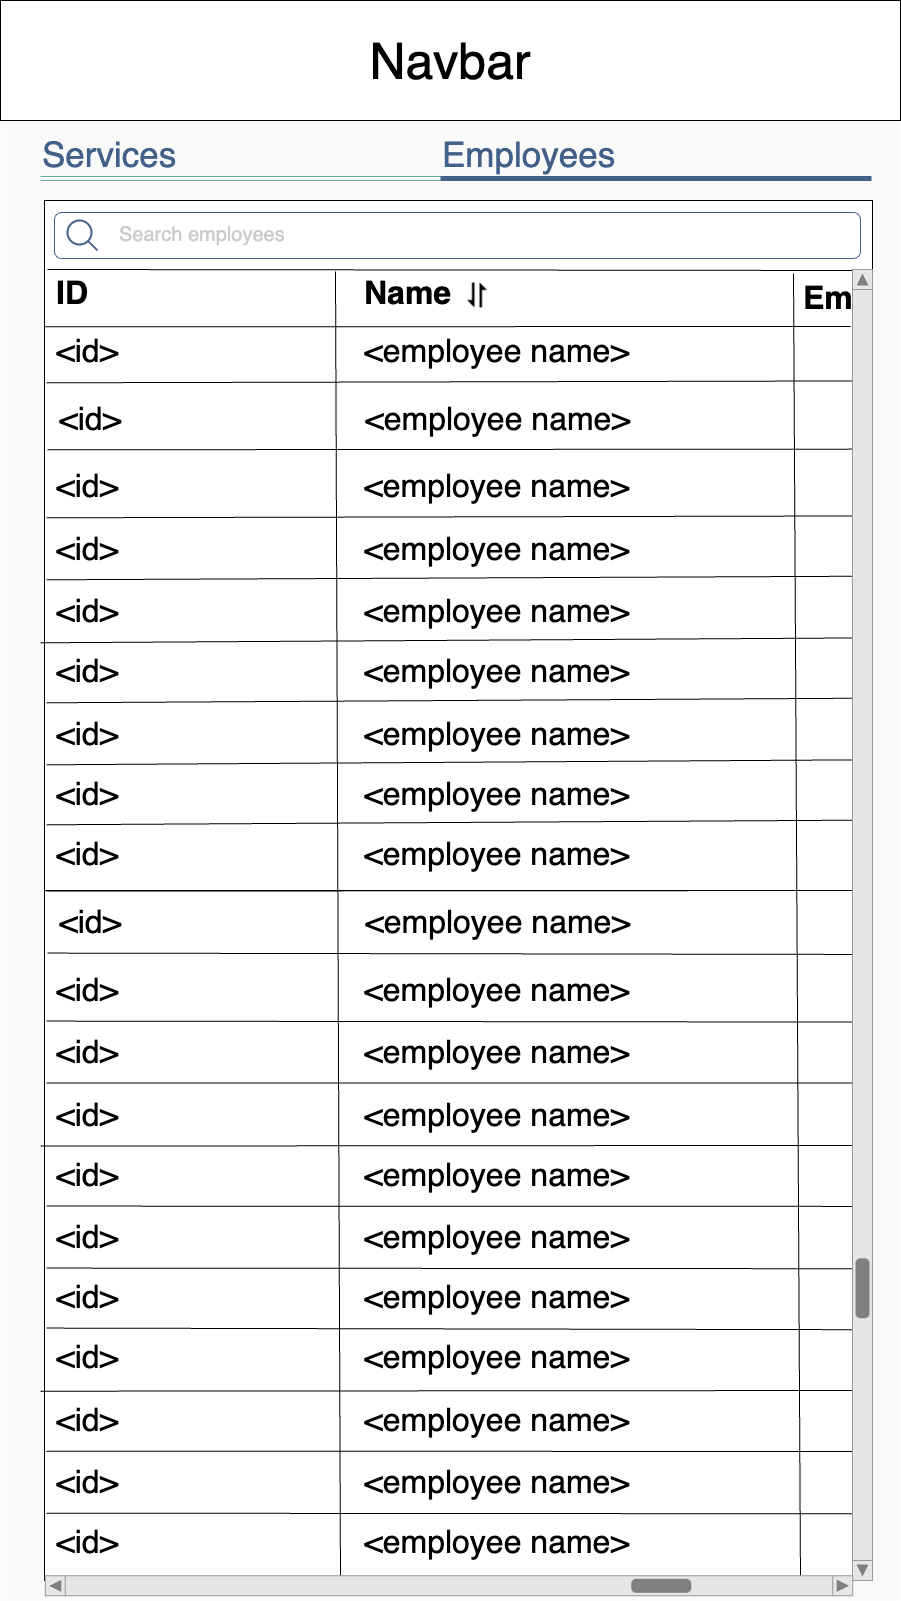
\includegraphics[width=0.5\textwidth]{mockups/Manage Shop (Employees) (Mobile).png}
	\caption{Manage Shop \textemdash{} Employees (Mobile)}
\end{figure}

\subsection{Manage Shop Details}

\begin{figure}[H]
	\centering
	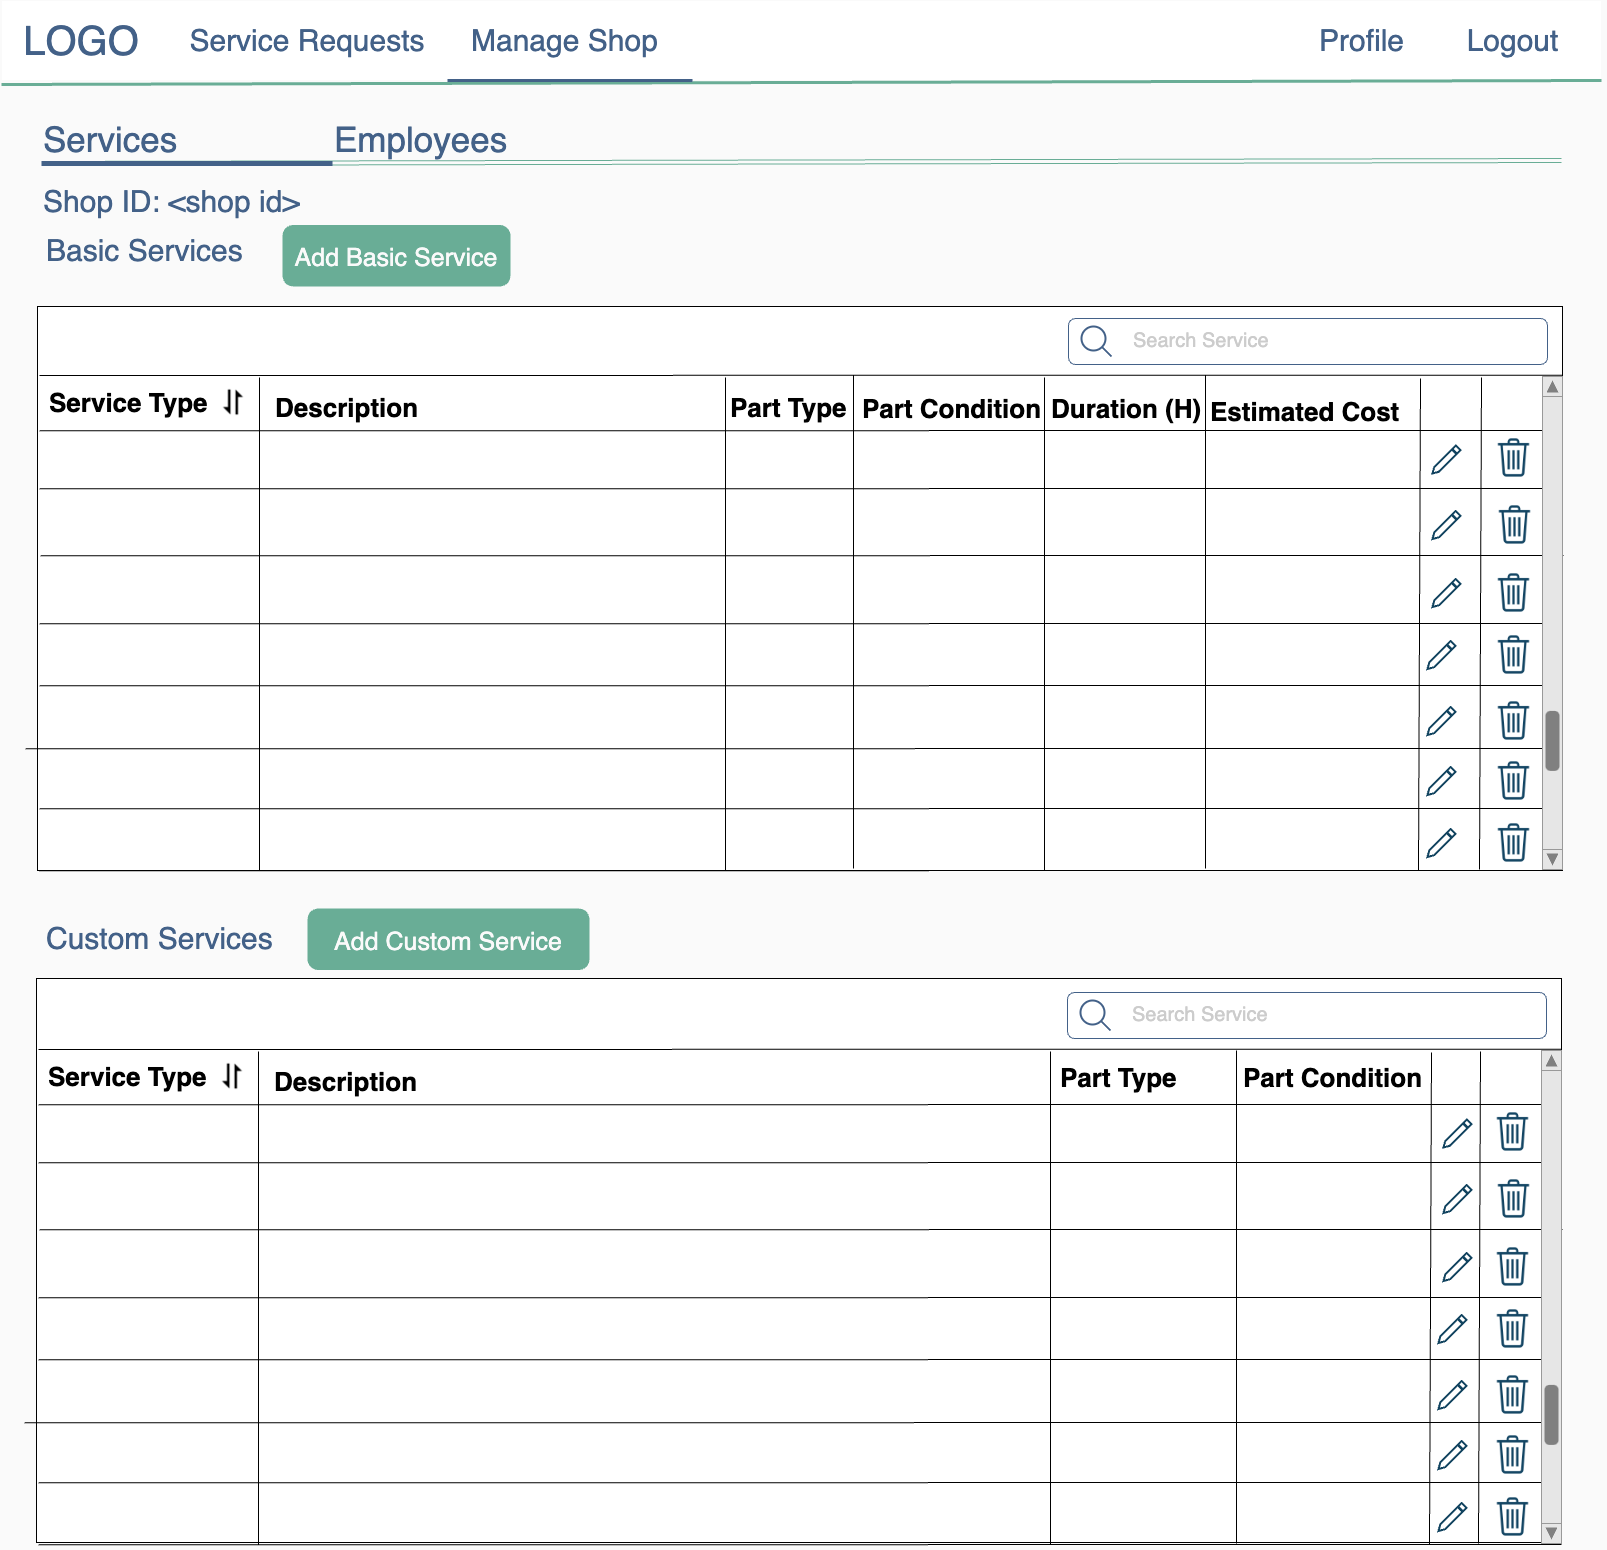
\includegraphics[width=\textwidth]{mockups/Manage Shop (Shop Settings) (Desktop).png}
	\caption{Manage Shop \textemdash{} Details (Desktop)}
\end{figure}

\begin{figure}[H]
	\centering
	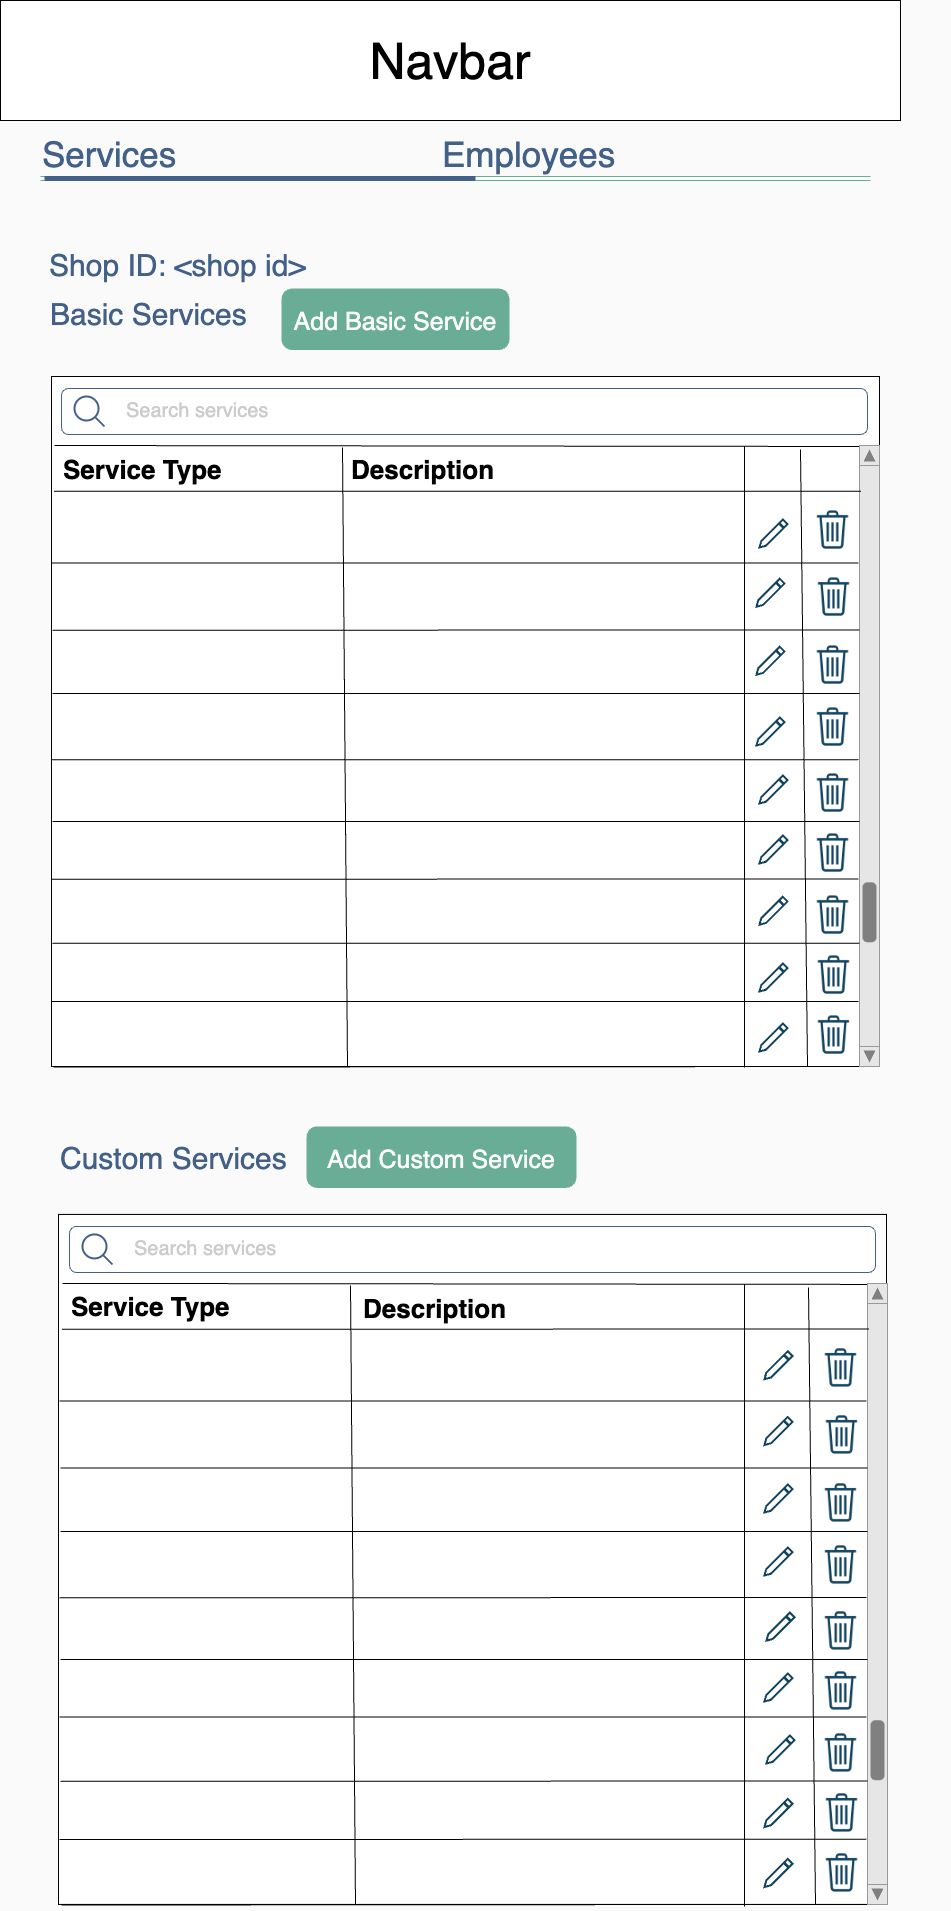
\includegraphics[width=0.5\textwidth]{mockups/Manage Shop (Shop Settings) (Mobile).png}
	\caption{Manage Shop \textemdash{} Details (Mobile)}
\end{figure}

\subsection{Work Orders}

\begin{figure}[H]
	\centering
	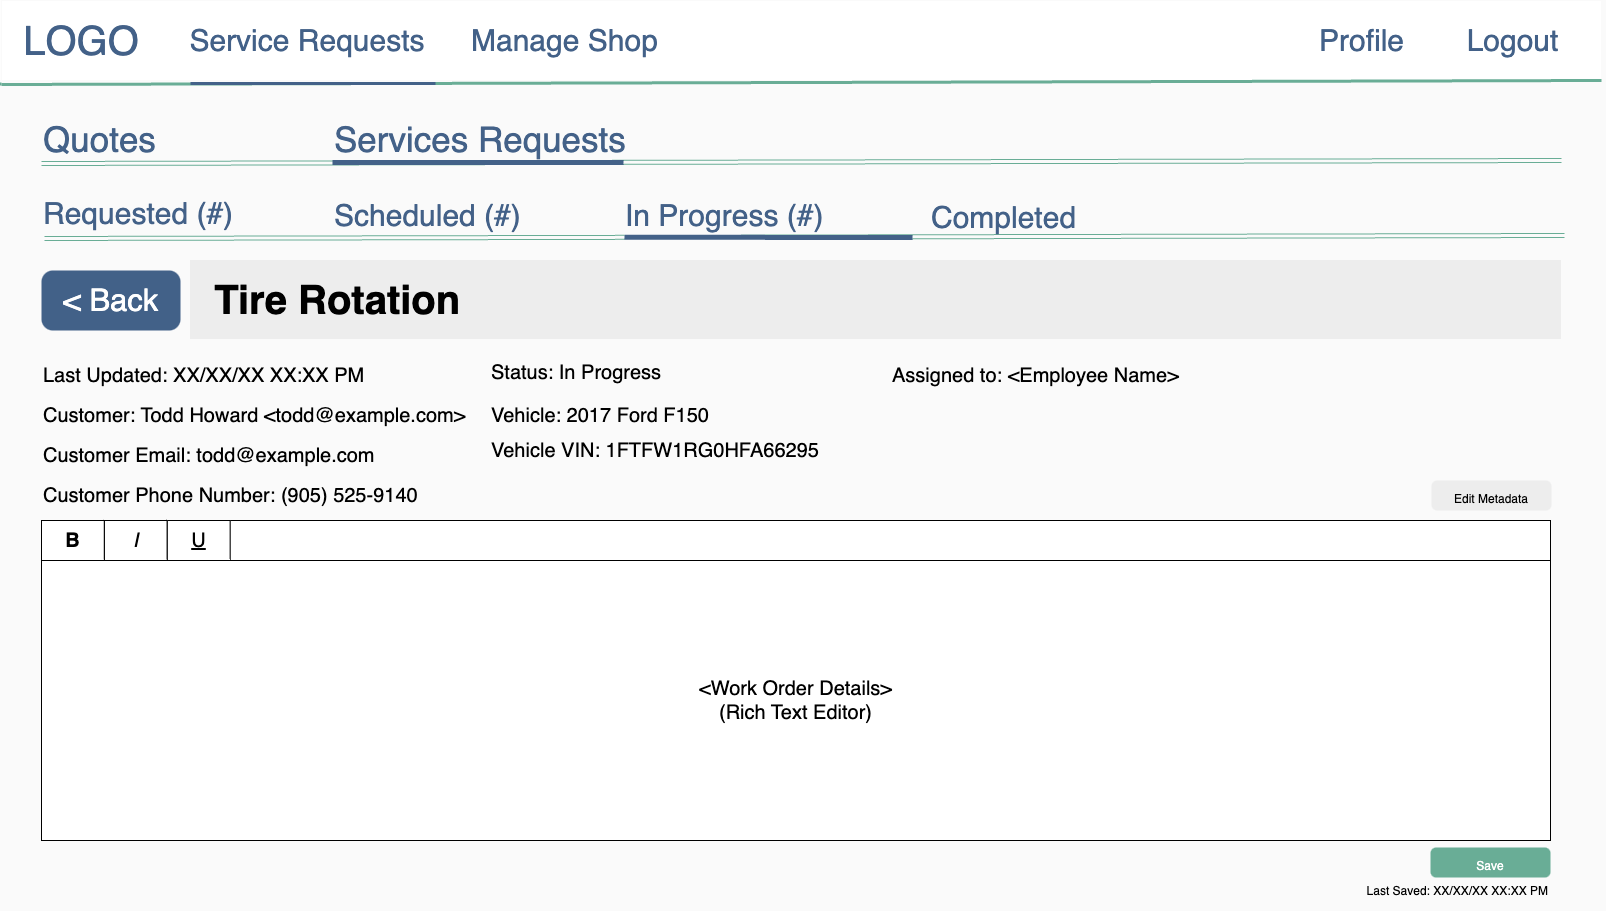
\includegraphics[width=\textwidth]{mockups/Shop Owner-Employee Work Order (Desktop).png}
	\caption{Work Orders (Desktop)}
\end{figure}

\begin{figure}[H]
	\centering
	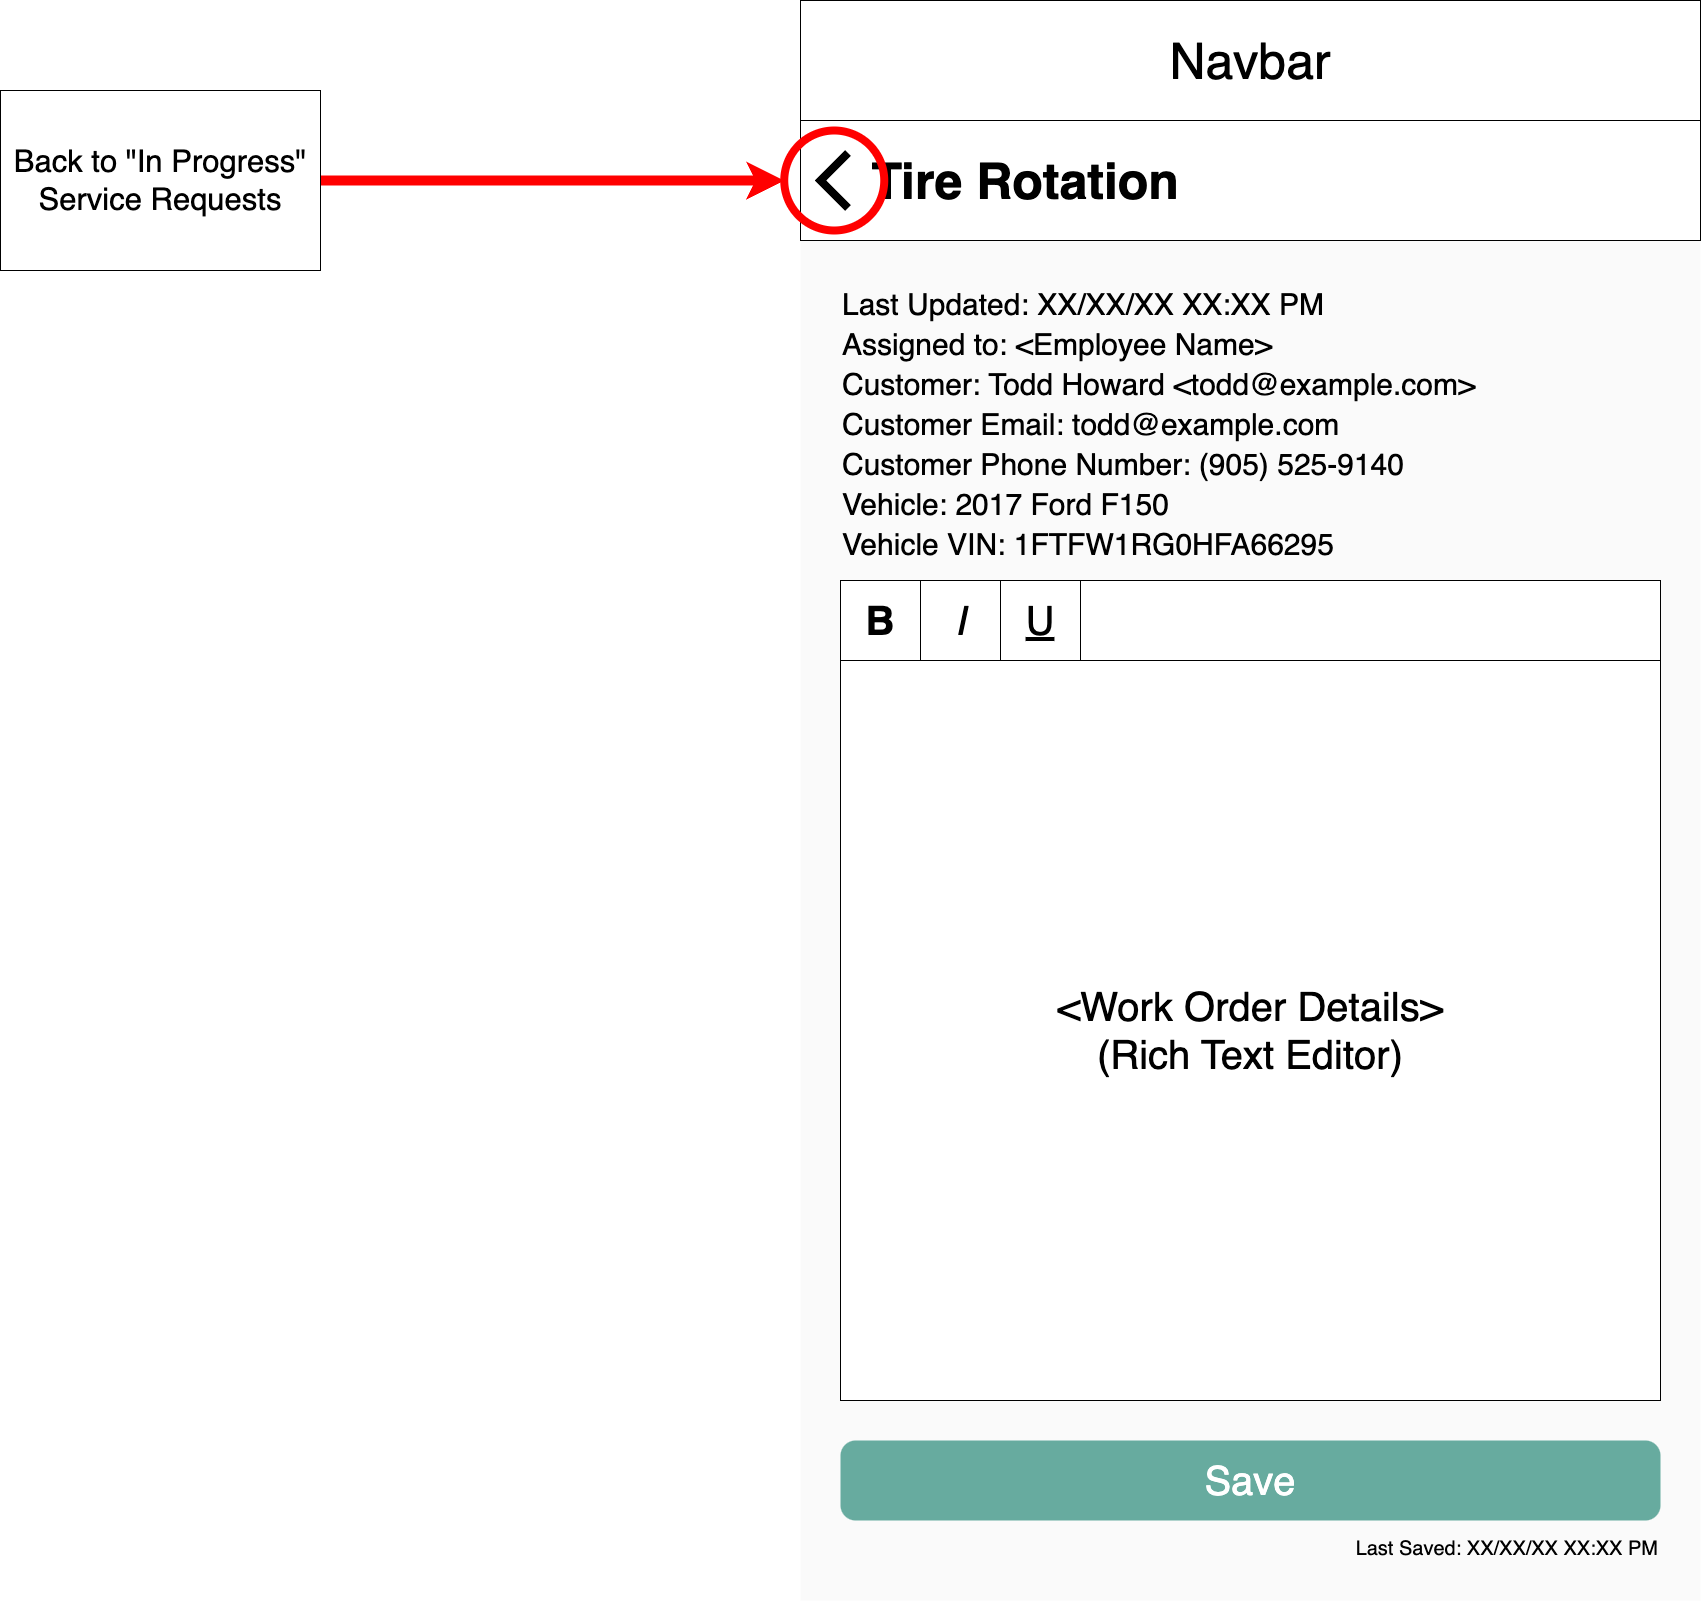
\includegraphics[width=\textwidth]{mockups/Shop Owner-Employee Work Order (Mobile).png}
	\caption{Work Orders (Mobile)}
\end{figure}

\section{Design of Hardware}
N/A

\section{Design of Electrical Components}
N/A

\section{Design of Communication Protocols}
N/A

\section{Timeline}

\subsection{Module Development}

The development of the modules shall take place over the months of December 2022 and January 2023.
Specific dates, and responsibilities are described in Table \ref{ModuleDevelopmentTimeline}.

\begin{table}[H]
	\caption{Module Development Timeline} \label{ModuleDevelopmentTimeline}
	\begin{tabular}{|p{0.32\textwidth}|p{0.4\textwidth}|p{0.23\textwidth}|}
		\hline
		\textbf{Module Name}       & \textbf{Development Timeline}             & \textbf{Developer(s)}    \\
		\hline
		Database Driver Module     & Dec. 1, 2022 \textemdash{} Jan. 31, 2023  & \makecell[l]{Arkin Modi, \\Joy Xiao,\\Leon So,\\Timothy Choy} \\
		\hline
		Users Module               & Dec. 1, 2022 \textemdash{} Dec. 15, 2022  & \makecell[l]{Arkin Modi, \\Leon So} \\
		\hline
		Employee Management Module & Dec. 15, 2022 \textemdash{} Dec. 22, 2022 & \makecell[l]{Joy Xiao,   \\Leon So} \\
		\hline
		Shop Module                & Dec. 15, 2022 \textemdash{} Dec. 22, 2022 & \makecell[l]{Leon So,    \\Timothy Choy} \\
		\hline
		Quotes Module              & Jan. 1, 2023 \textemdash{} Jan. 8, 2023   & \makecell[l]{Arkin Modi, \\Timothy Choy} \\
		\hline
		Services Module            & Jan. 1, 2023 \textemdash{} Jan. 8, 2023   & \makecell[l]{Arkin Modi, \\Joy Xiao} \\
		\hline
		Appointments Module        & Jan. 15, 2023 \textemdash{} Jan. 22, 2023 & \makecell[l]{Arkin Modi, \\Joy Xiao,\\Timothy Choy} \\
		\hline
		Work Orders Module         & Jan. 15, 2023 \textemdash{} Jan. 24, 2023 & Arkin Modi               \\
		\hline
	\end{tabular}
\end{table}

\subsection{Module Testing}

The testing of the modules shall take place over the months of December 2022 and January 2023. The
tests conducted shall primarily consist of manual testing and have the primary goal of certifying
confidence for the Revision 0 Demonstration. This testing will not include everything described in
the System Verification and Validation Plan. Generally, testing will take place for the week after
development is scheduled to finish. Specific dates, and responsibilities are described in Table
\ref{ModuleTestingTimeline}.

\begin{table}[H]
	\caption{Module Testing Timeline} \label{ModuleTestingTimeline}
	\begin{tabular}{|p{0.32\textwidth}|p{0.4\textwidth}|p{0.23\textwidth}|}
		\hline
		\textbf{Module Name}       & \textbf{Testing Timeline}                 & \textbf{Developer(s)}    \\
		\hline
		Database Driver Module     & Dec. 1, 2022 \textemdash{} Jan. 31, 2023  & \makecell[l]{Arkin Modi, \\Joy Xiao,\\Leon So,\\Timothy Choy} \\
		\hline
		Users Module               & Dec. 15, 2022 \textemdash{} Dec. 22, 2022 & \makecell[l]{Arkin Modi, \\Leon So} \\
		\hline
		Employee Management Module & Dec. 22, 2022 \textemdash{} Dec. 29, 2022 & \makecell[l]{Joy Xiao,   \\Leon So} \\
		\hline
		Shop Module                & Dec. 22, 2022 \textemdash{} Dec. 29, 2022 & \makecell[l]{Leon So,    \\Timothy Choy} \\
		\hline
		Quotes Module              & Jan. 8, 2023 \textemdash{} Jan. 15, 2023  & \makecell[l]{Arkin Modi, \\Timothy Choy} \\
		\hline
		Services Module            & Jan. 8, 2023 \textemdash{} Jan. 15, 2023  & \makecell[l]{Arkin Modi, \\Joy Xiao} \\
		\hline
		Appointments Module        & Jan. 22, 2023 \textemdash{} Jan. 29, 2023 & \makecell[l]{Arkin Modi, \\Joy Xiao,\\Timothy Choy} \\
		\hline
		Work Orders Module         & Jan. 24, 2023 \textemdash{} Jan. 31, 2023 & Arkin Modi               \\
		\hline
	\end{tabular}
\end{table}

% \newpage
% \bibliographystyle {plainnat}
% \bibliography{../../../refs/References}

\newpage

\section{Appendix}

\subsection{Interface}

\wss{Include additional information related to the appearance of, and
	interaction with, the user interface}

\subsection{Reflection}

The information in this section will be used to evaluate the team members on the graduate attribute
of Problem Analysis and Design. Please answer the following questions:

\begin{enumerate}
	\item What are the limitations of your solution? Put another way, given unlimited resources, what could
	      you do to make the project better? (LO\_ProbSolutions)
	\item Give a brief overview of other design solutions you considered. What are the benefits and tradeoffs
	      of those other designs compared with the chosen design? From all the potential options, why did you
	      select documented design? (LO\_Explores)
\end{enumerate}

\end{document}
